\documentclass[]{article}
\usepackage{amsmath}
\usepackage{tabularx}
\usepackage{graphicx}
\usepackage{caption}
\captionsetup{labelformat=empty,labelsep=none}
\title{Priming Experiments on Linguistic Enrichment}
\author{Ishan Somshekar | SUID: ishans}
\date{}
\begin{document}
\maketitle

\section*{Linguistic Enrichment}

When a listener parses a sentence, they will often derive meaning not just from what is spoken, but also what is left unsaid. This additional implied meaning arises from the listener's trust that the speaker is adhering to certain maxims of conversation. As Grice(1975) laid out, if the listener trusts that the speaker will (1) make their contribution truthful, (2) be as informative as required, (3) be relevant, and (4) be brief, the listener can successfully gain additional information. \\
For example, in the sentences below:\\
\\
1. Some of the children are in the classroom.\\
		\textit{Not all of the children are in the classroom}\\
Here we see that the listener will imply that 'some' means 'not all', as even though the sentence would be true if all children were in the room, the listener trusts that if all children were already in the room, the speaker would have said 'all' instead of some.\\
\\
2. I've got two children.\\
		\textit{I don't have more than two children}\\
Example 2 shows a similar linguistic enrichment in the case of numerals, where the fact that the speaker has said 'two' children leads the listener to believe that the speaker does not have more than two children.\\
\\
There are in general two types of interpretations for sentences in any enrichment category: a strong interpretation and a weak interpretation. I will now shortly discuss the different interpretations that can arise for the two categories of enrichment that this experiment will examine.\\
\\
The first category of enrichment relates to the 'some' quantifier. The strong interpretation of 'some' is 'not all', i.e. when a speaker chooses to use the word 'some', they are doing so because the statement would not be true if 'some' was replaced by 'all'. In a weak interpretation, the meaning of some is taken to be 'any amount'. \\
\textit{'When some of the children come back to class, I'll close the window.'}\\
In this sentence, we are supposed to take the weak interpretation, as a strong interpretation would suggest that the speaker would close the window when some children return but reopen it when all have returned, which wouldn't make much sense. \\
\\
The second category of enrichment relates to numeric values. In this experiment, we will explore the use of 'four' and 'six'. The strong interpretation of these numerics is 'exactly', based on the listener's assumption that the speaker is being as informative as necessary. In a weak interpretation, the meaning of the numeric is taken to be 'at least'.\\
\textit{Parents with two children are eligible for child support.}\
In this sentence, we are supposed to again take the weak interpretation, as we should substitute 'at least' into the sentence for the correct interpretation.\\
\\
It is important to note that the correct strength (strong/weak) of interpretation necessary is not just dependent on the structure of the sentence, but also some inherent qualities of the category. We can see in following sentences that we take the strong interpretation for the numeric enrichment category, but the weak for the quantifier enrichment category, even though the sentences are otherwise the same.\\
\textit{“Everyone who took some of their anti-allergy pills felt fine”} \\
\textit{“Everyone who took two of their anti-allergy pills felt fine”} \\
\\

\section*{Priming Hypothesis}
Lewis Bott and Emmanuel Chemla, in their 2016 paper \textit{Shared and distinct mechanisms in deriving linguistic enrichment}, attempt to produce priming effects for these different categories of linguistic enrichment. \\
Priming effects occur when "participants adopt a particular linguistic structure on one trial (the prime) and then adopt the same structure on a subsequent trial (the target)."\footnote{Bott and Chemla 2016, p.120.} Chemla and Bott hypothesize that one could construct an experiment where the strong or weak interpretations of enrichment categories could be primed.\\
There are two different hypothesis that they initial paper sets forth with regards to the possible existence of priming in enrichment categories.\\
\\Firstly, if a strong prime of a category results in a higher proportion of strong target responses in that category than a weak prime, then this is evidence for structural priming in this category of linguistic enrichment.
\\Second, If a strong prime of a category results in a higher proportion of strong target responses in a different category, this would be evidence for enrichment mechanisms that exist outside of sentence specifics, as the priming effect on enrichment is existing across different sentence types, so it must be an alternative mechanism that is being primed.\\


\section*{Methods}
\subsection*{Experiment Details}
The general form of the experiment involved the use of Priming trials followed by Target trials. Each trial (Prime or Target) consisted of a single descriptor sentence with two card images underneath. Participants were prompted to choose the card that they felt best suited their interpretation of the descriptor sentence.\\
The following three images are example slides that were shown to participants at the beginning of each experiment to familiarize them with this format.
There were two types of priming trials: strong primes and weak primes. The strong prime trials had a descriptor sentence, a card for which the weak interpretation of the sentence was true, and a card for which the strong interpretation (and thus also the weak interpretation) was true. In this case, the correct response to the priming trial would be to select the strong interpretation card.\\
The weak prime trials had a descriptor sentence, a card for which the weak interpretation was true, and a card that the descriptor sentence did not match with (a false interpretation). In this case, the correct response to the priming trial was to select the weak interpretation card.\\
Target trials had a descriptor sentence, a card for which the weak interpretation was true, and a card that simply read 'Better Image?', which the participants could choose if they were not satisfied by the weak interpretation of the image.\\
\\
The following three images are example slides that the participants were shown to familiarize themselves with the framework.\\
\begin{figure}[h]

\centering
\begin{minipage}[b]{0.3\textwidth}
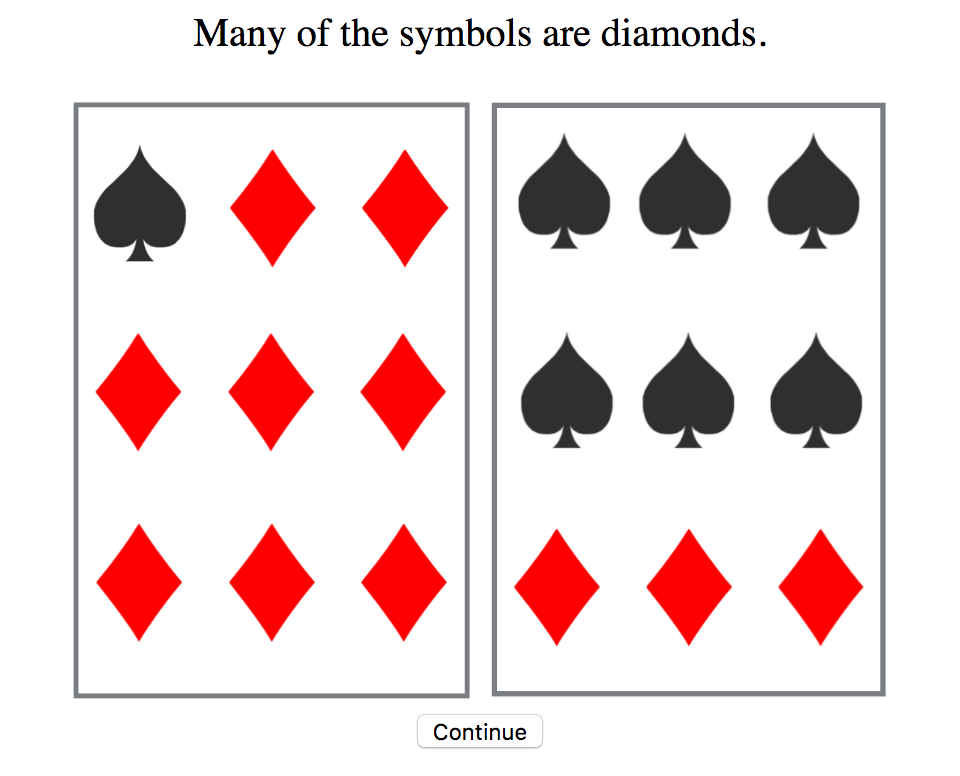
\includegraphics[width=\textwidth]{example1.png} 
\end{minipage}
\begin{minipage}[b]{0.3\textwidth}
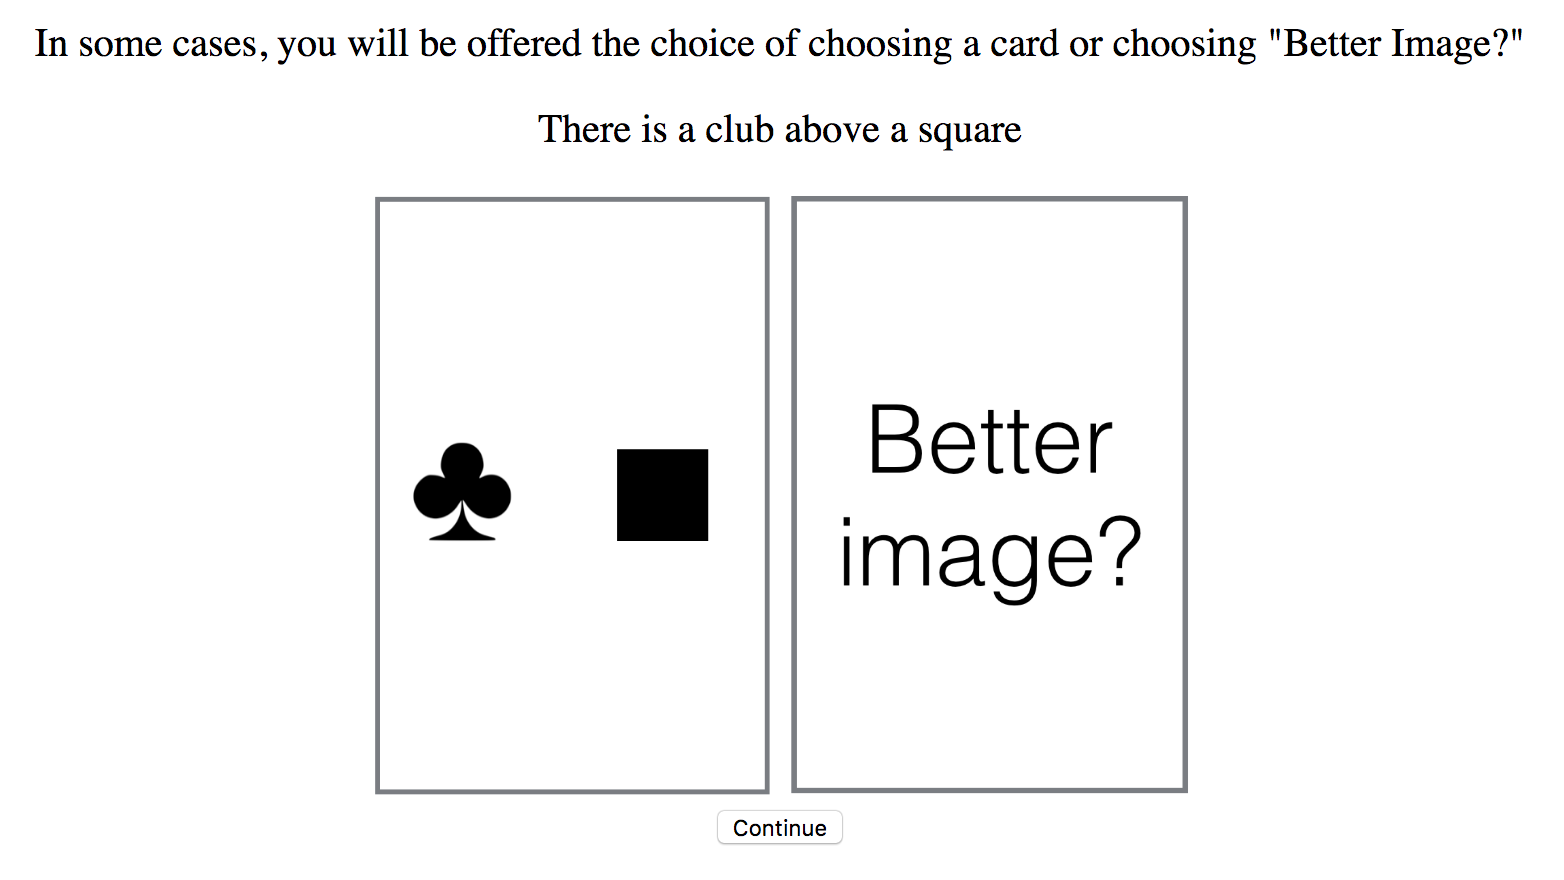
\includegraphics[width=\textwidth]{example2.png} 
\end{minipage}
\begin{minipage}[b]{0.3\textwidth}
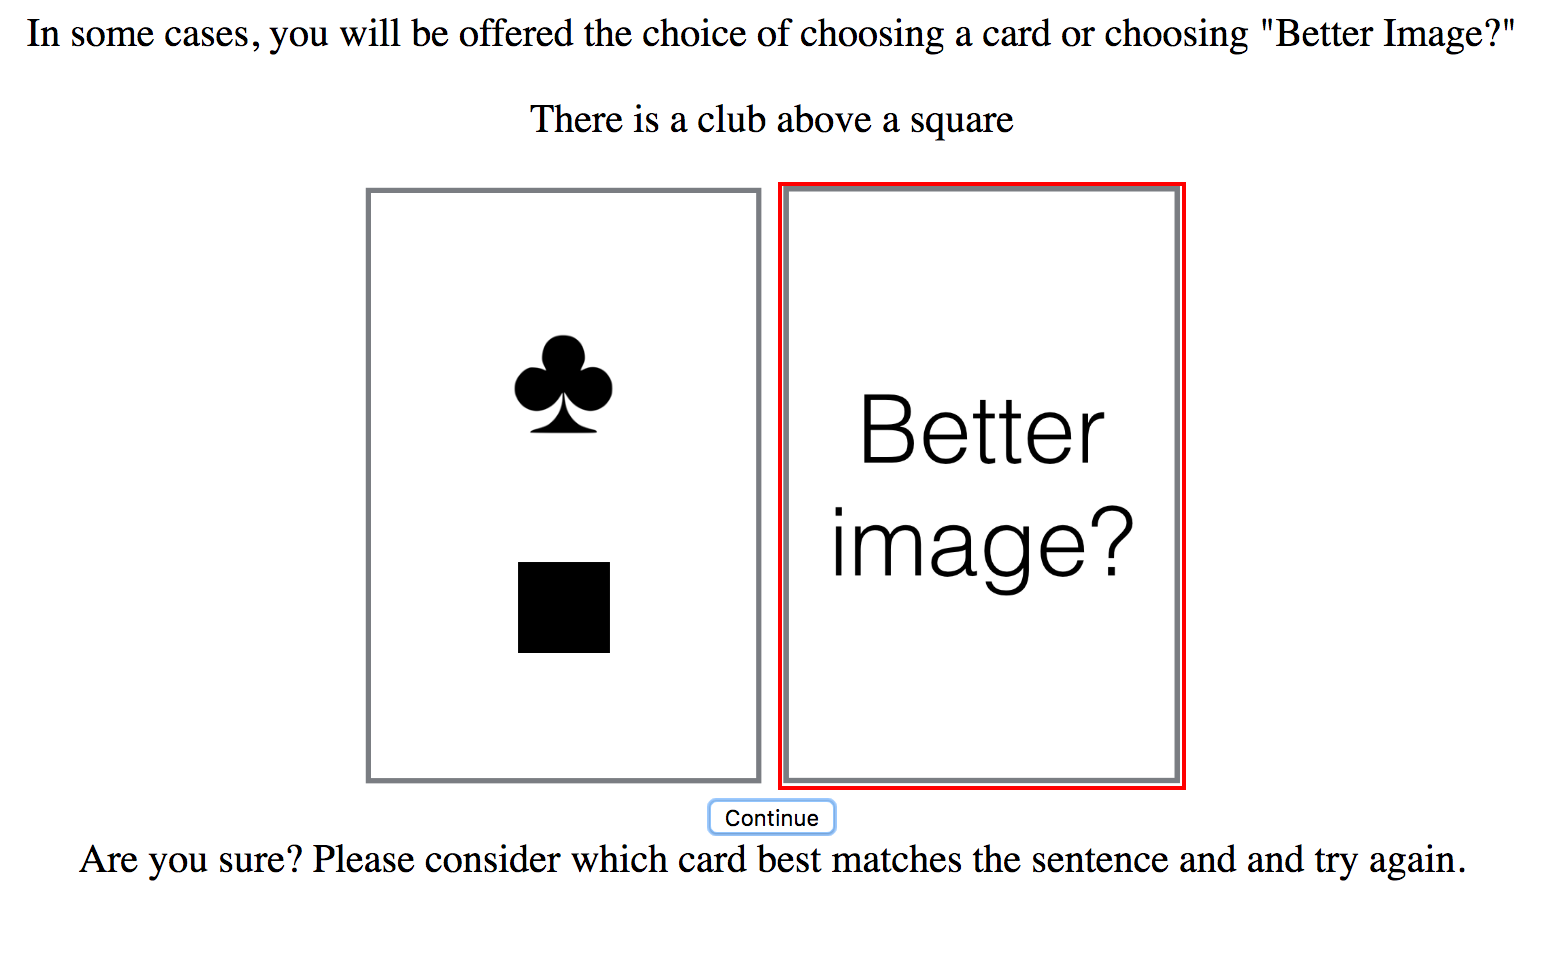
\includegraphics[width=\textwidth]{example3.png} 
\end{minipage}
\end{figure}
\pagebreak

The experiment tested priming within the enrichment category for quantifiers with 'some' and the the enrichment category for numerals with 'four' and 'six'.\\
The following figures showcase the strong prime/weak prime/target trials for each of the enrichment categories.\\
\begin{figure}[h]
\centering
\begin{minipage}[b]{0.3\textwidth}
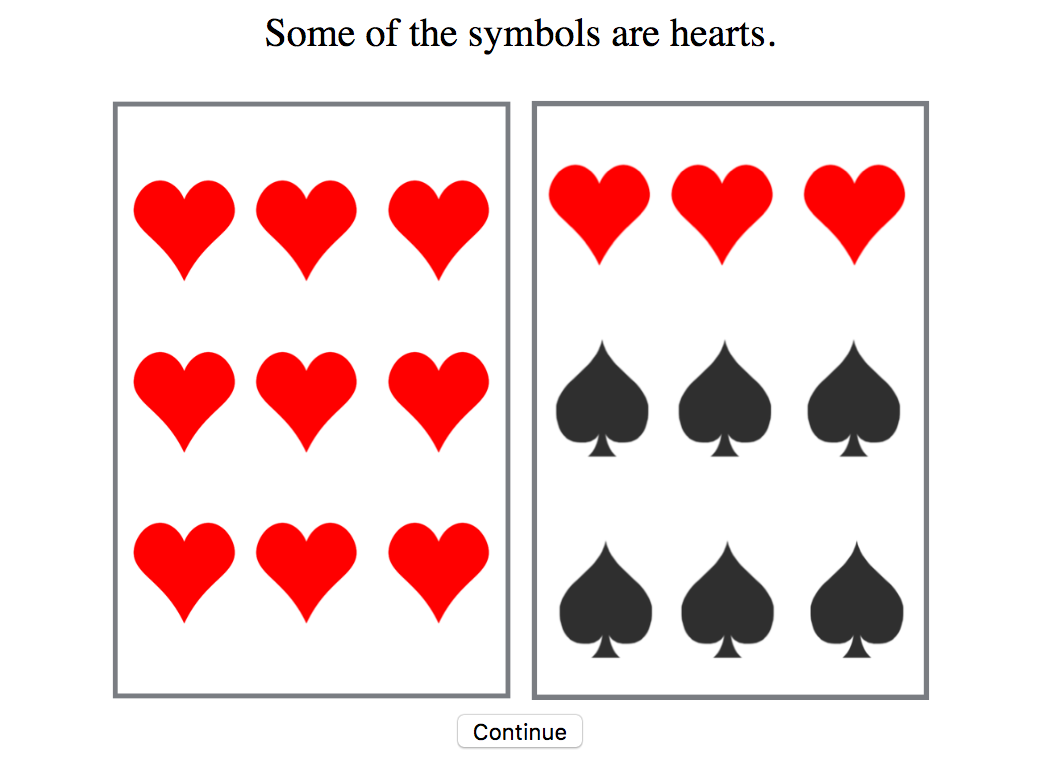
\includegraphics[width=\textwidth]{some_strong.png} 
\caption{'some' strong prime}
\end{minipage}
\begin{minipage}[b]{0.3\textwidth}

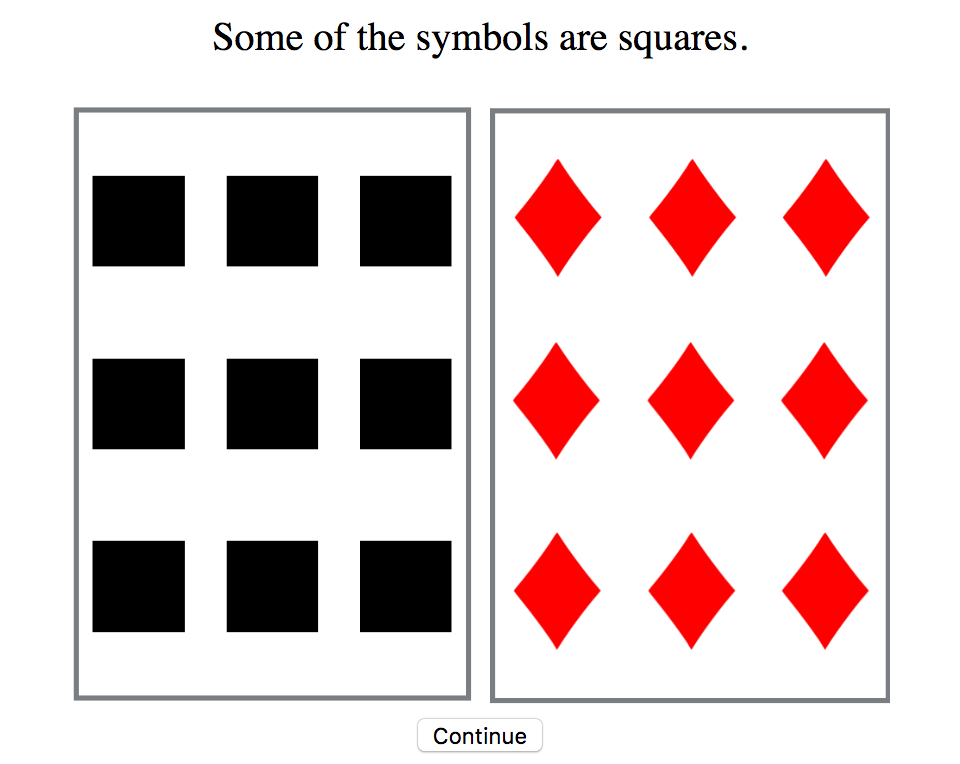
\includegraphics[width=\textwidth]{some_weak.png} 
\caption{'some' weak prime}
\end{minipage}
\begin{minipage}[b]{0.3\textwidth}

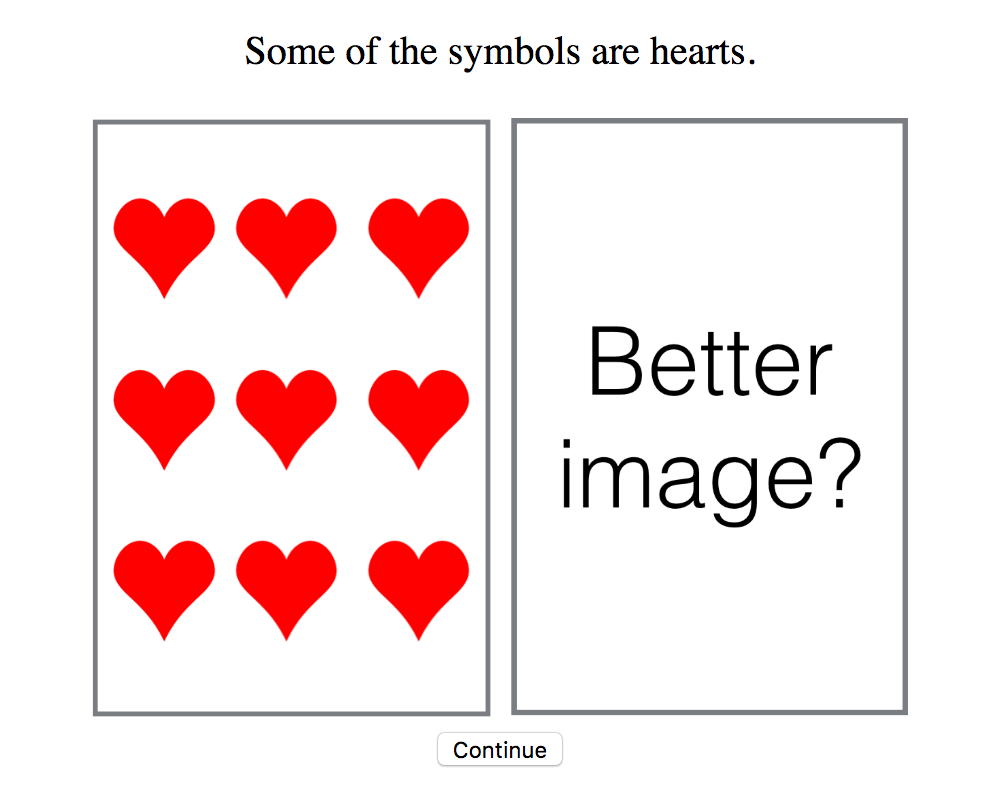
\includegraphics[width=\textwidth]{some_test.png} 
\caption{'some' target }
\end{minipage}
\end{figure}

\begin{figure}[h]
\centering
\begin{minipage}[b]{0.3\textwidth}
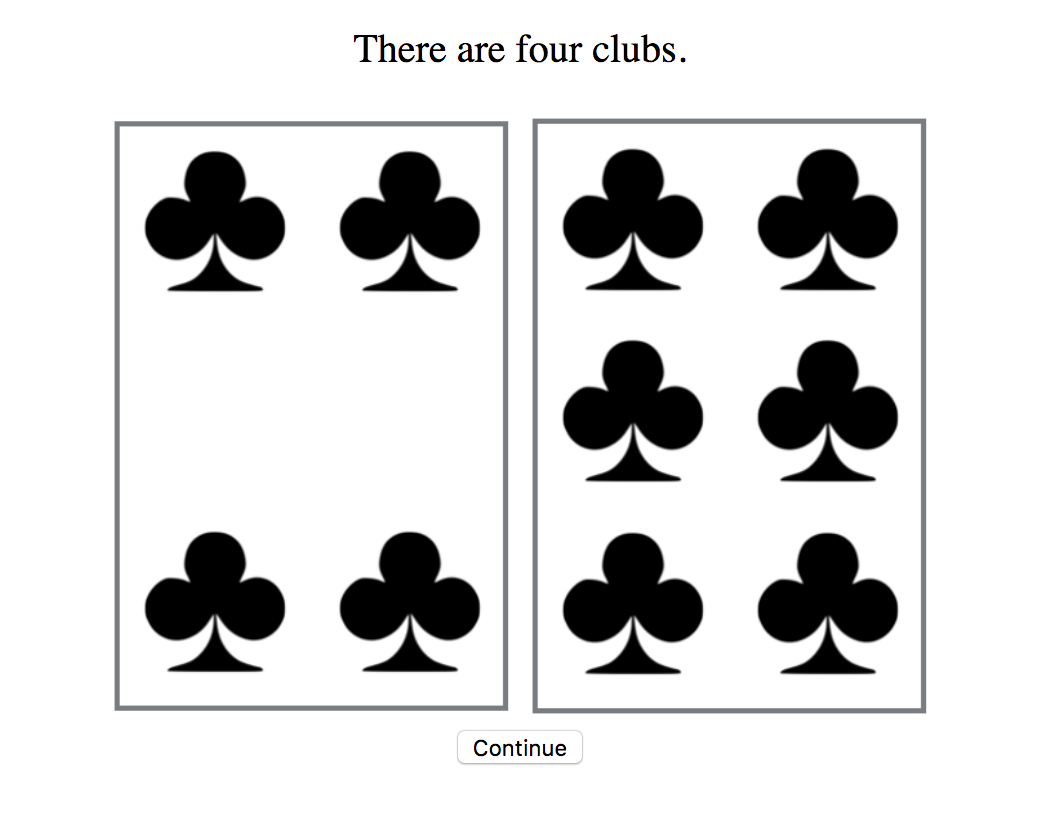
\includegraphics[width=\textwidth]{four_strong.png} 
\caption{'four' strong prime}
\end{minipage}
\begin{minipage}[b]{0.3\textwidth}

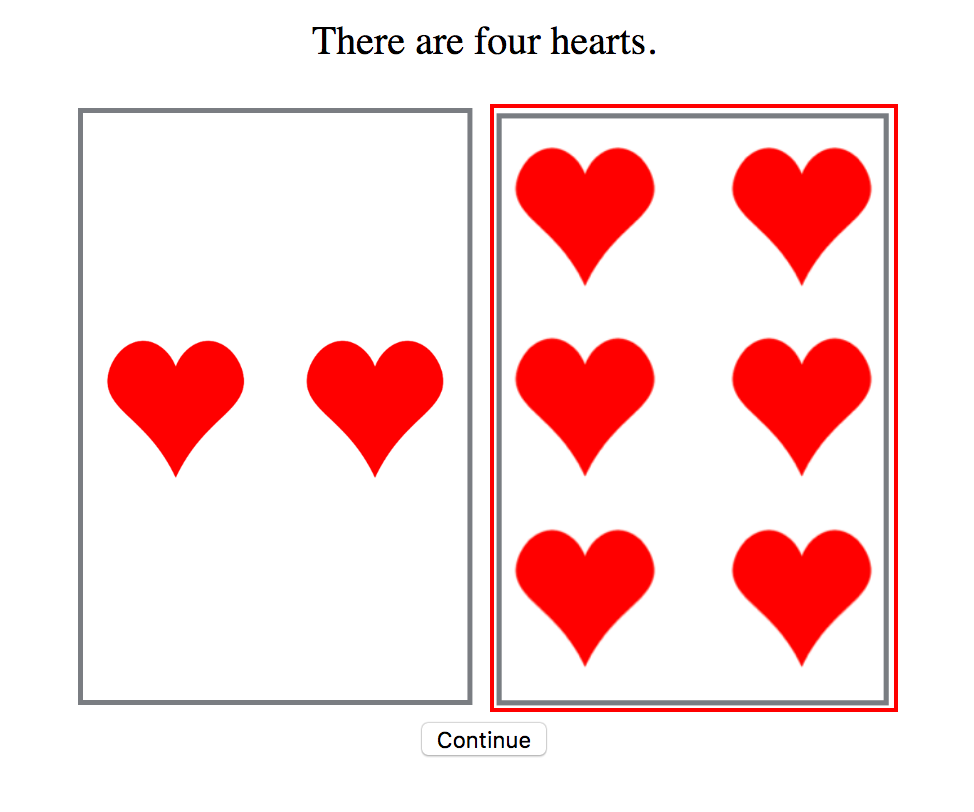
\includegraphics[width=\textwidth]{four_weak.png} 
\caption{'four' weak prime}
\end{minipage}
\begin{minipage}[b]{0.3\textwidth}

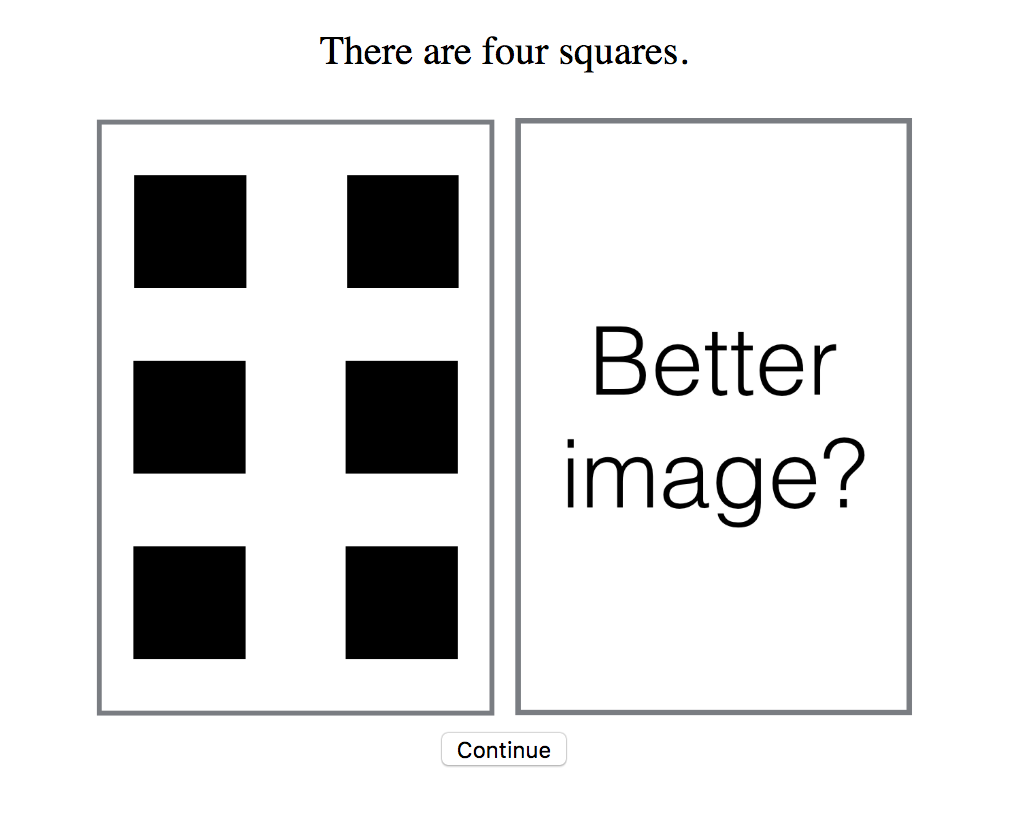
\includegraphics[width=\textwidth]{four_test.png} 
\caption{'four' target }
\end{minipage}
\end{figure}

\begin{figure}[h]
\centering
\begin{minipage}[b]{0.3\textwidth}
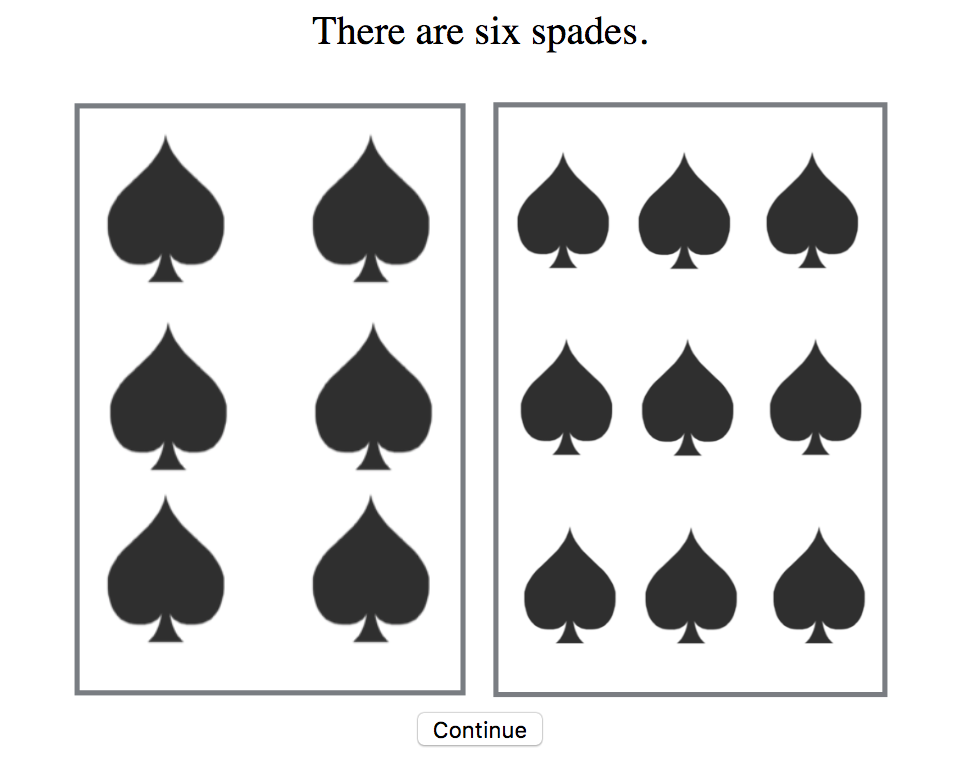
\includegraphics[width=\textwidth]{six_strong.png} 
\caption{'six' strong prime}
\end{minipage}
\begin{minipage}[b]{0.3\textwidth}

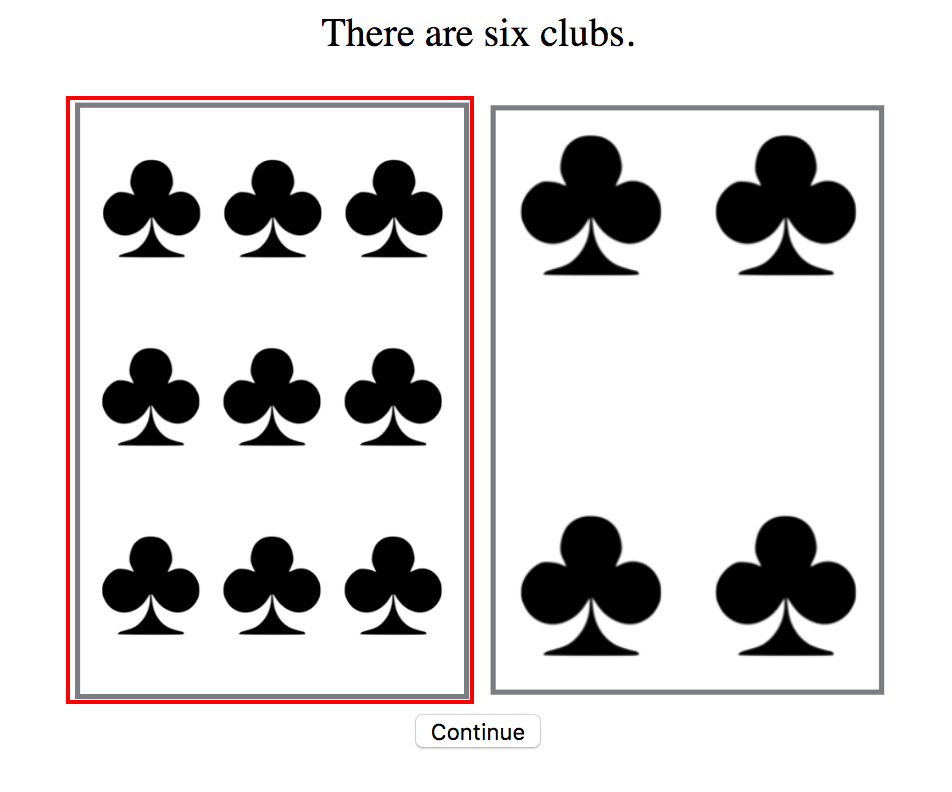
\includegraphics[width=\textwidth]{six_weak.png} 
\caption{'six' weak prime}
\end{minipage}
\begin{minipage}[b]{0.3\textwidth}

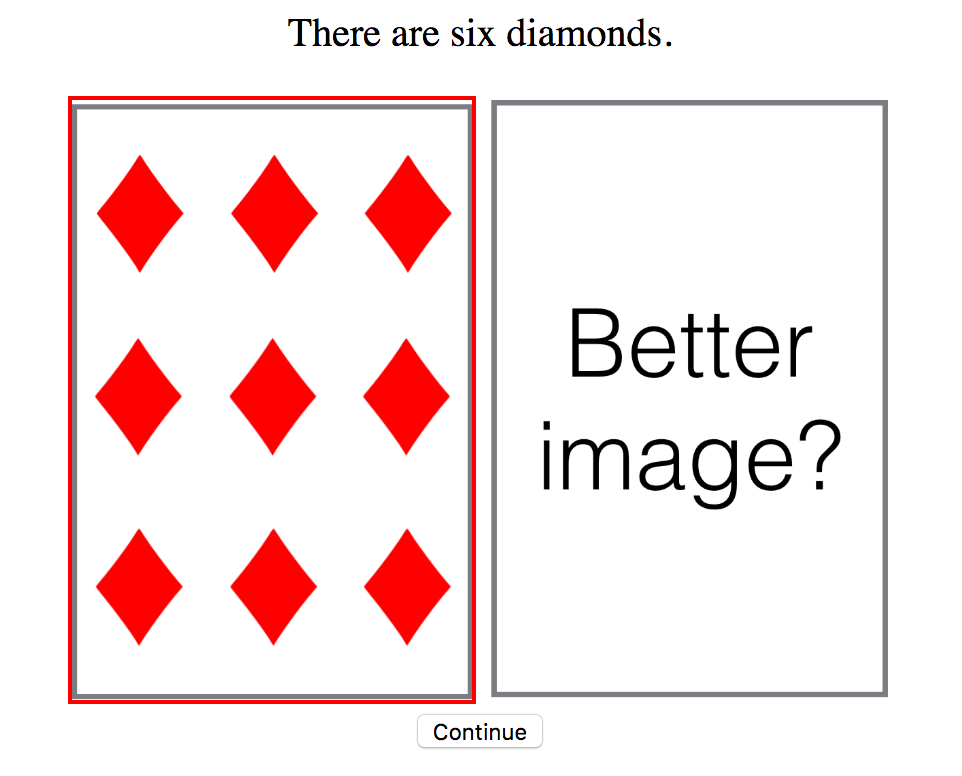
\includegraphics[width=\textwidth]{six_test.png} 
\caption{'six' target }
\end{minipage}
\end{figure}

Each complete trial consisted of two prime trials of the same enrichment category and strength, followed by a target trial. These sets were fully crossed, there were complete trials in which the prime trials and the target trial matched in enrichment category, and trials where they did not.\\
\\
 As a result, there were $3 \text{(enrichment category of prime trials)} * 2 \text{(prime strength)} * 3 \text{(enrichment category of target)} = 18$ different types of complete trials. \\
The experiment had 3 of each complete trial, so each participant saw 54 complete trials in our replication. Our replication also had 12 filler trials which were not considered in the results, for a total of 66 trials. \\
The full experiment had 4 sets of each complete trial and 12 filler trials, our replication was smaller due to financial constraints for compensation of participants.\\
The order of the trials was completely randomized for each participant, and the selection of shapes for each card (heart, diamond, spade, club, square) was also completely randomized.



\subsection*{Participants}
40 participants were recruited for this trial through the use of Mechanical Turk. 
I decided to exclude any participant who produced an incorrect response to any of the priming trials and any participant who did not list English as their native language. However, no participants failed these conditions, so data from all 40 was considered in the final set. 

\subsection*{Procedure}
Each participant was asked to click on the card that best matched the sentence and then press the continue button (or the space bar) for each of the $(66*3) = 198$ slides in the experiment.

\pagebreak
\section*{Results}
For each type of trial (prime enrichment category)x(prime strength)x(target enrichment category), we measured the proportion of responses in the target trial that were a strong response. Strong responses implied that the participant had taken a strong interpretation of the target trial descriptor sentence, and clicked on better image.\\

We can see the results in this visualization here. Each pair of (prime enrichment category type x trial enrichment category type) has  columns (strong and weak) that represent the proportion of strong target trial responses following a pair of strong primes or weak primes respectively.\\

We can see that the within category priming (some-some , four-four, six-six) are very different from the across category priming results. The two areas that stand out are four-four and some-some; in these cases we can clearly see that a strong prime produces a higher proportion of strong responses than a weak prime.

\begin{figure}[h]
\centering
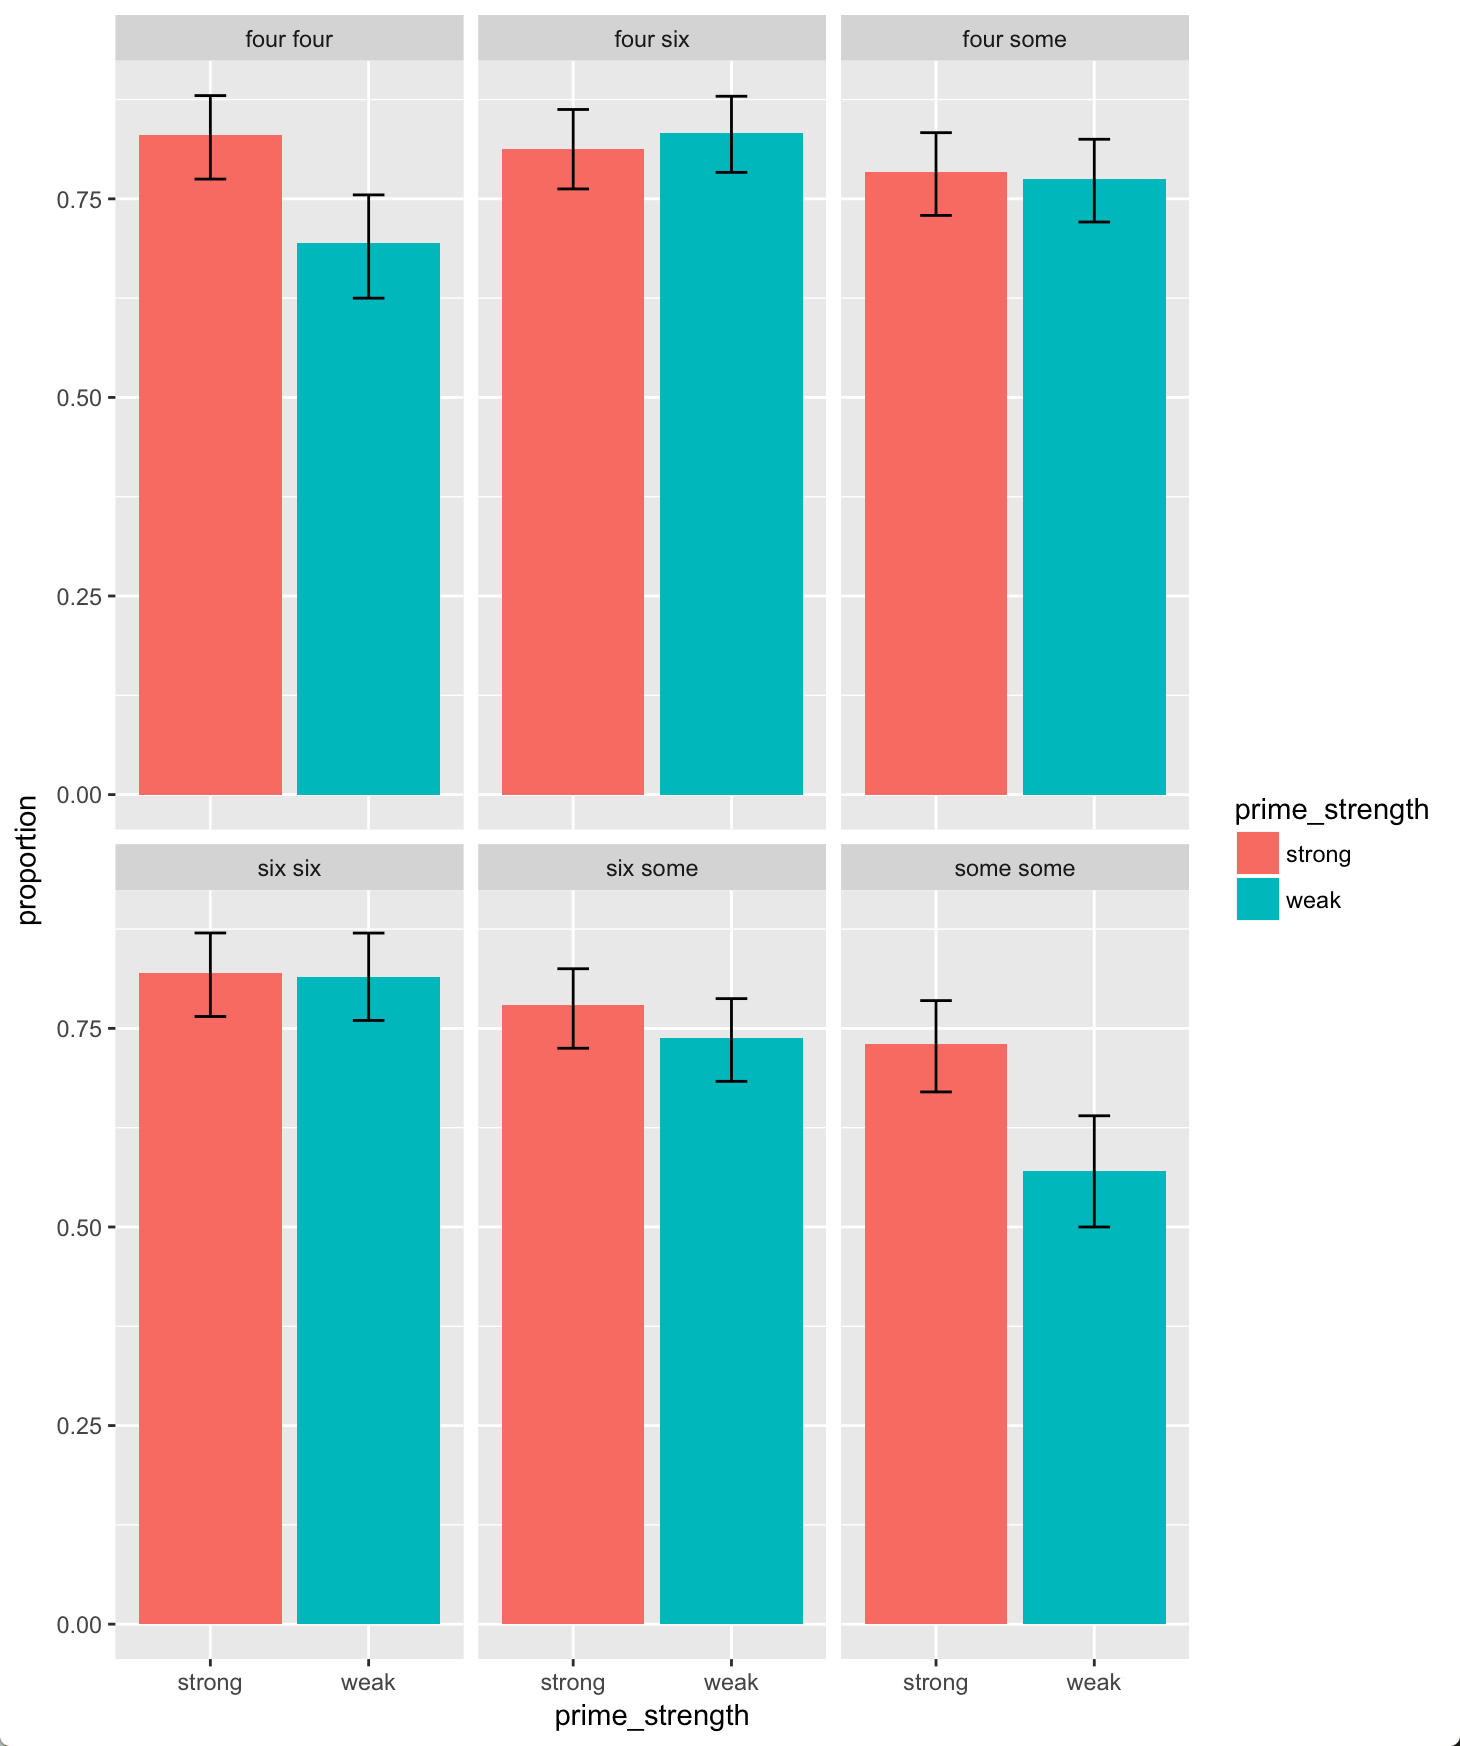
\includegraphics[scale=0.3]{results.png} 
\end{figure}

We can also use logistic regression mixed effect models, which were modeled in R, to see what effects arise from the data. In the tables below, the R-pseudocode for a model is followed by the results for that same model. 
\pagebreak

The first model we can fit is a logistic regression model on all the data. Here we see that there is a strong effect of prime strength, such that a weak prime would result in a lower percentage of strong responses. This effect is increased when we limit to the within category priming, as the interaction between withinBetween-within and primeStrength-weak shows a greater B-value.
\begin{table}[h]
\caption{$strongResponse \sim 1 + primeStrength*withinBetween +(1 + primeStrength*withinBetween | workerID)$}
\begin{center}
\begin{tabularx}{1.1\textwidth}{|X c c c c|}
\hline 
effect & $\beta$ & Std. error & z-value & $Pr(>|z|)$ \\
\hline
primeStrengthweak & -0.7445 & 0.3750 & -1.986 & 0.0471* \\

withinBetweenwithin & -0.2630 & 0.3682 & -0.714 & 0.4750 \\

primeStrengthweak:withinBetweenwithin & -0.8273 & 0.4202 & -1.969 &  0.0490*\\
\hline
\end{tabularx}
\end{center}
\end{table}

Since the visualization of the results showed that we seemed to be achieving better priming in the within-category, we can try and fit a model using only the data from within trials.

In this model, we see that the effect of primeStrength-weak is much greater.
\begin{table}[h]
\caption{$strongResponse \sim 1 + primeStrength*primeCategory +(1 + primeStrength*primeCategory | workerID)$}
\begin{center}
\begin{tabularx}{1.1\textwidth}{|X c c c c|}
\hline 
effect & $\beta$ & Std. error & z-value & $Pr(>|z|)$ \\
\hline
primeStrength-weak &  -2.4205 & 0.8401 & -2.881 & 0.00396 ** \\
primeType-six & 1.6311 & 1.7259 & 0.945 & 0.34463 \\
primeType-some & -1.8982 & 0.9245 & -2.053 & 0.04006 *  \\
primeStrength-weak:primeType-six & 0.9143 & 1.9956 &  0.458 & 0.64683\\
primeStrength-weak:primeType-some & 0.6160 & 0.9534 & 0.646 & 0.51825 \\    

\hline
\end{tabularx}
\end{center}
\end{table}

\section*{Discussion}
The overall results were similar to those gotten by Bott and Chemla, but I was unable to perfectly replicate their results. There was a higher proportion of strong responses in the replication than in the original in every single combination of category-prime strength. Upon analysing individual participant's responses further, I found that of the 40 participants, 24 selected the strong response over 85\% of the time. It is likely that the original authors saw something similar, but the effect may have been less prominent over 200 participants.\\
\\
Bott and Chemla produced evidence for enrichment priming in all three of the within-trials (some-some, four-four, and six-six). In this replication, while strong primes produced a higher proportion of strong responses for 'four' and 'some', there was no similar effect for 'six'. This was particularly strange; I think that this may have arisen to some issue with the replication or just an unfortunate skew of data, because it does not make much sense for two of the within category trials to be successful and one to fail. Returning to our initial hypotheses, I think that these results are enough to suggest that the first hypothesis is true: we can show evidence for priming for a specific category of enrichment. \\
\\
The replication was unable to reproduce the between category priming exhibited in the original paper. Bott and Chemla were able to show real effects of between category priming; our replication did not produce those effects. In our replication, strong primes did not generally produce a higher proportion of strong responses than weak primes did between categories of enrichment. Again, this is dissimilar to the original paper. \\ 
While I do think that there could be the chance that we can produce priming effects across enrichment categories, and thus validate our second hypothesis, this particular experimental set up leaves me with a few questions. Firstly, it seems that there should be a difference between the between category of 'four-six' and 'four-some', as one is changing the value of a numeral within the numerals enrichment category, and the other is moving from numerals to quantifiers. Also, Bott and Chemla combine both directions in their analysis (four->six and six->four are combined). I would have liked to see them broken apart, as looking at the combined data may be hiding trends that are specific to just one direction, or broadcasting trends of one direction to both directions.\\
\\
To conclude, even though the replication was able to reproduce the same results as the original paper, I do think the second hypothesis, that there can exist mechanisms for interpreting enrichment that are outside sentence specifics, intuitively makes sense. Humans should definitely be able to build a 'speaker identity' that would lean towards weak(or strong) interpretations depending on the speaker. Due to the encoded randomness, this experiment is not conducive to building that type of speaker identity, and that could be one of the reasons why we could not replicate the between category results that would depend on identity of that form. \\
\\
\pagebreak
\section*{References}
 \begin{enumerate}
 \item Bott Lewis \& Chemla, Emmanuel. (2016). Shared and distinct mechanisms in deriving linguistic enrichment.\textit{Journal of Memory and Language, 91}. 117-140.
 \item Grice, H. Paul. (1989). Studies in the Way of Words.
\end{enumerate} 

\end{document}

